\ifgerman{\chapter{Grundlagen und verwandte Arbeit}}{\chapter{Background and Related Work}}
\label{background}

%- Allgemeine Wissensgrundlagen des Fachgebiets
%- Spezielle Grundlagen, die für das Verständnis erforderlich sind
%- Rahmenbedingungen für die Arbeit
%- Ausführungen zum Stand des Wissens / der Technik
%Als Leitprinzip gilt: Nur Informationen erwähnen, die
%- später benötigt werden,
%- notwendig sind, um die Arbeit oder ihre Motivation zu verstehen
%Das heißt insbesondere,
%- keine Inhalte aus Lehrbüchern, außer
%- diese werden benötigt, um Problemstellung oder Lösungsweg zu definieren.

The main focus of this work is the estimation of classifier performance in the special case of an active learning scenario. To help better understand the problem setting, we will give a brief overview of the concepts of active learning as well as an in-depth look of existing methods for said estimation. We also establish parts of the notation that will be used for the remainder of this work.

\section{Classification}
Many problems to be solved encompass the differentiation between certain "classes" to which their inputs can be assigned. To explain the concept of \textbf{classification}, we assume the example of a thermostat. Its purpose is to monitor the temperature in a certain area and fire up a heating unit to raise the temperature if necessary. But for that to happen, the thermostat has to \textit{classify} the measured temperature in the categories "too cold" and "warm enough". In this special case a simple threshold usually suffices. Generally, however, a \textit{classifier} $C$ is defined as a mapping of a \textit{feature vector}, also called an \textit{instance}, to its corresponding \textit{class label} $y \in Y = \{y_1, ..., y_m\}$. It is convenient to describe said vector as an n-tuple of \textit{feature values}: $\vec{x} = (x_1, ..., x_n)$ with $x_i \in F_i$ $\forall i=\{1,...,n\}$ and $F_i$ as a \textit{feature}. The goal of a classifier is to approximate the underlying "true" association of a feature vector to its class label $f(\vec{x}) = y$, which can be written as
\begin{equation}
C: F_1 \times ... \times F_n \rightarrow Y
\end{equation}
or $\hat{f}(\vec{x}) = \hat{y}$ \cite{RodriguezEtAl2013}. This definition makes it clear that classification is not restricted to single-variable problems. To stick with our example of a thermostat, you may want to consider the humidity, temperature outdoors or whether any windows are open to decide if heating is necessary. Closely related are \textit{regression problems}. While a classifier works with discrete class labels, regression uses a continuous output space.

To obtain a classifier for a specific problem, one makes use of what is called a \textit{learning algorithm} $A$. In a process called \textit{training} a set of instances, the \textit{training data} $X_T = \{(\vec{x}_1, y_1), ..., (\vec{x}_n, y_n)\}$, is taken and such a mapping $C$ using an optimization criterion is created. The training set is a subset of a distribution of all possible data and should be independently and identically distributed. The whole data set can be modeled as a bivariate distribution with the feature vectors and class labels as random variables: $(\mathbf{X}, \mathbf{Y})$ \cite{RodriguezEtAl2013}. While all learning algorithms are being fed feature vectors to create a classifier, they can be separated into three categories, depending on their requirement for labeling:
\begin{itemize}
\item \textbf{Supervised:}
This type of algorithm requires all of their input data to be labeled as well as a list of all possible class labels. While it may seem like the best option, its drawbacks include the potential cost of the labeling. If the correct class labels are not inherently known, usually a human is required to assign the correct labels manually. With unlabeled data readily available for problems like speech recognition, this is a very expensive part of the process. Another issue is the propagation of errors; any mistake made during labeling is carried over into the modeling of the classifier.

\item \textbf{Unsupervised:}
Instead of requiring all data to be labeled, unsupervised algorithms ignore class labels completely. This saves the cost of labeling the data, but many algorithms require some sort of tuning parameters (e.g. the cardinality of $Y$ and shape of underlying probability distribution).

\item \textbf{Semi-supervised:}
As a compromise of the two extremes, semi-supervised techniques operate with a mix of labeled and unlabeled data. This way it seeks to combine the low effort for labeling with the advantages of supervised learning \cite{ZhuEtAl2009}.
\end{itemize}

Regardless of their category, all learning methods make assumptions about the distribution of the data: feature vectors close to each other tend to belong to the same class and, consequently, data points are likely to form group-like structures.

\section{Active learning}
As a subgroup of semi-supervised learning, active learners try to optimize the performance of a classifier when using a fixed amount of class labels. To achieve this, they make the training an iterative process, selecting one or more instances for labeling that the believe will benefit the performance the most in each iteration. While more exist, we will touch on three of them here:

\subsection{Random sampling}
This active learner is the baseline for all other ones. It does not show a preference for any instance, hence its name, making at is good or bad as not using active learning at all.

\subsection{Uncertainty sampling}
The \textit{uncertainty} of a classifier with regard to an instance describes how sure it is about the class label it would assign. This can be measured in various ways, three of which are:

\begin{itemize}
\item \textbf{Least confidence}:
This measure assumes that the instance for which the classifier produces the lowest probability estimate for its most likely class label $\hat{y}$ has the highest uncertainty $u$ \cite{CulottaEtAl2004}:
\begin{equation}
u_{LC}(\vec{x}) = 1 - P_c(\hat{y} | \vec{x})
\end{equation}
\item \textbf{Smallest margin}:
Here the difference in probability between the \textit{two} most likely class labels $y_1, y_2$ for an instance is used as the uncertainty measure \cite{SchefferEtAl2001}:
\begin{equation}
u_{SM}(\vec{x}) = P_c(y_1 | \vec{x}) - P_c(y_2 | \vec{x})
\end{equation}
\item \textbf{Maximum entropy}:
Instead of only using the probability of a few class labels, the entropy takes all of them into account \cite{DaganEtAl1995}:
\begin{equation}
u_{ME}(\vec{x}) = -\sum_{y}^{} P_c(y | \vec{x}) \cdot log_2(P_c(y | \vec{x}))
\end{equation}
It should be noted that, while they possibly select different instances in multi-class problems, the first two are numerically identical for dichotomous data and all three will select the same instance \cite{ZhuEtAl2008}. In any case, they all assume what is called a \textit{decision boundary}, an entity which spatially separates groups of instances sharing the same class label. This can problematic if multiple clusters of the same label exist, as they are likely to be regarded as if they would belong to a different group.
\end{itemize}

\subsection{Probabilistic Active Learning (PAL)}
PAL takes a different approach. It takes a look at each available instance's surroundings and computes the density of unlabeled as well as the amount of already purchased instances. The latter combined with the portion of instances sharing their class label with the original instance is denoted as \textit{label statistics}. Using this, assuming the instance's class label and the overall probability of this class in its neighbourhood was to be known, an optimal selection with regard to the classifier's performance could be made. But since those two quantities are generally unknown, PAL considers them as random variables. This enables the computation of an expected or probabilistic performance gain for each unlabeled instance. When weighted with the instance density in its neighbourhood, it allows an statistically optimal selection for the performance \cite{KremplEtAl2014}.

\begin{figure}[h]
	\centering
	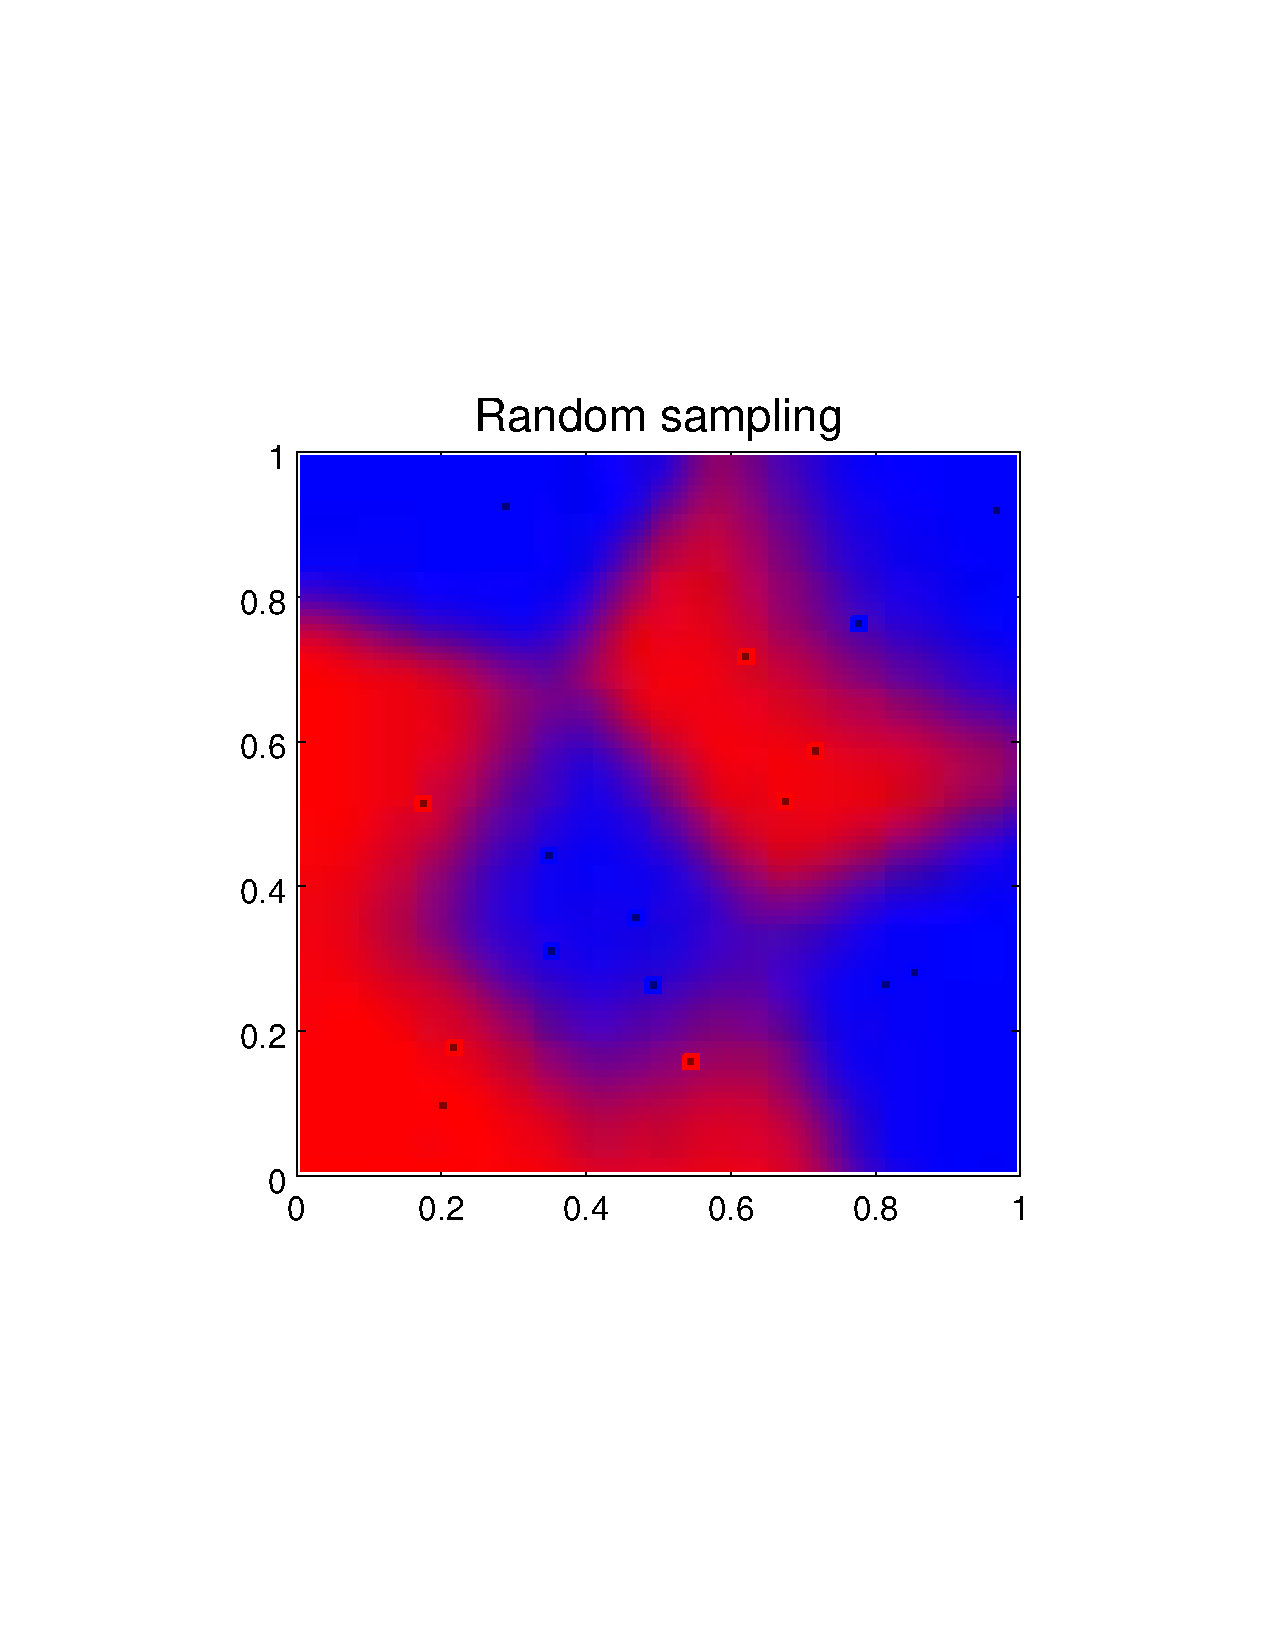
\includegraphics[trim = 4cm 6cm 4cm 4cm, clip = true, width = 0.253\textwidth]{RS16inst}
	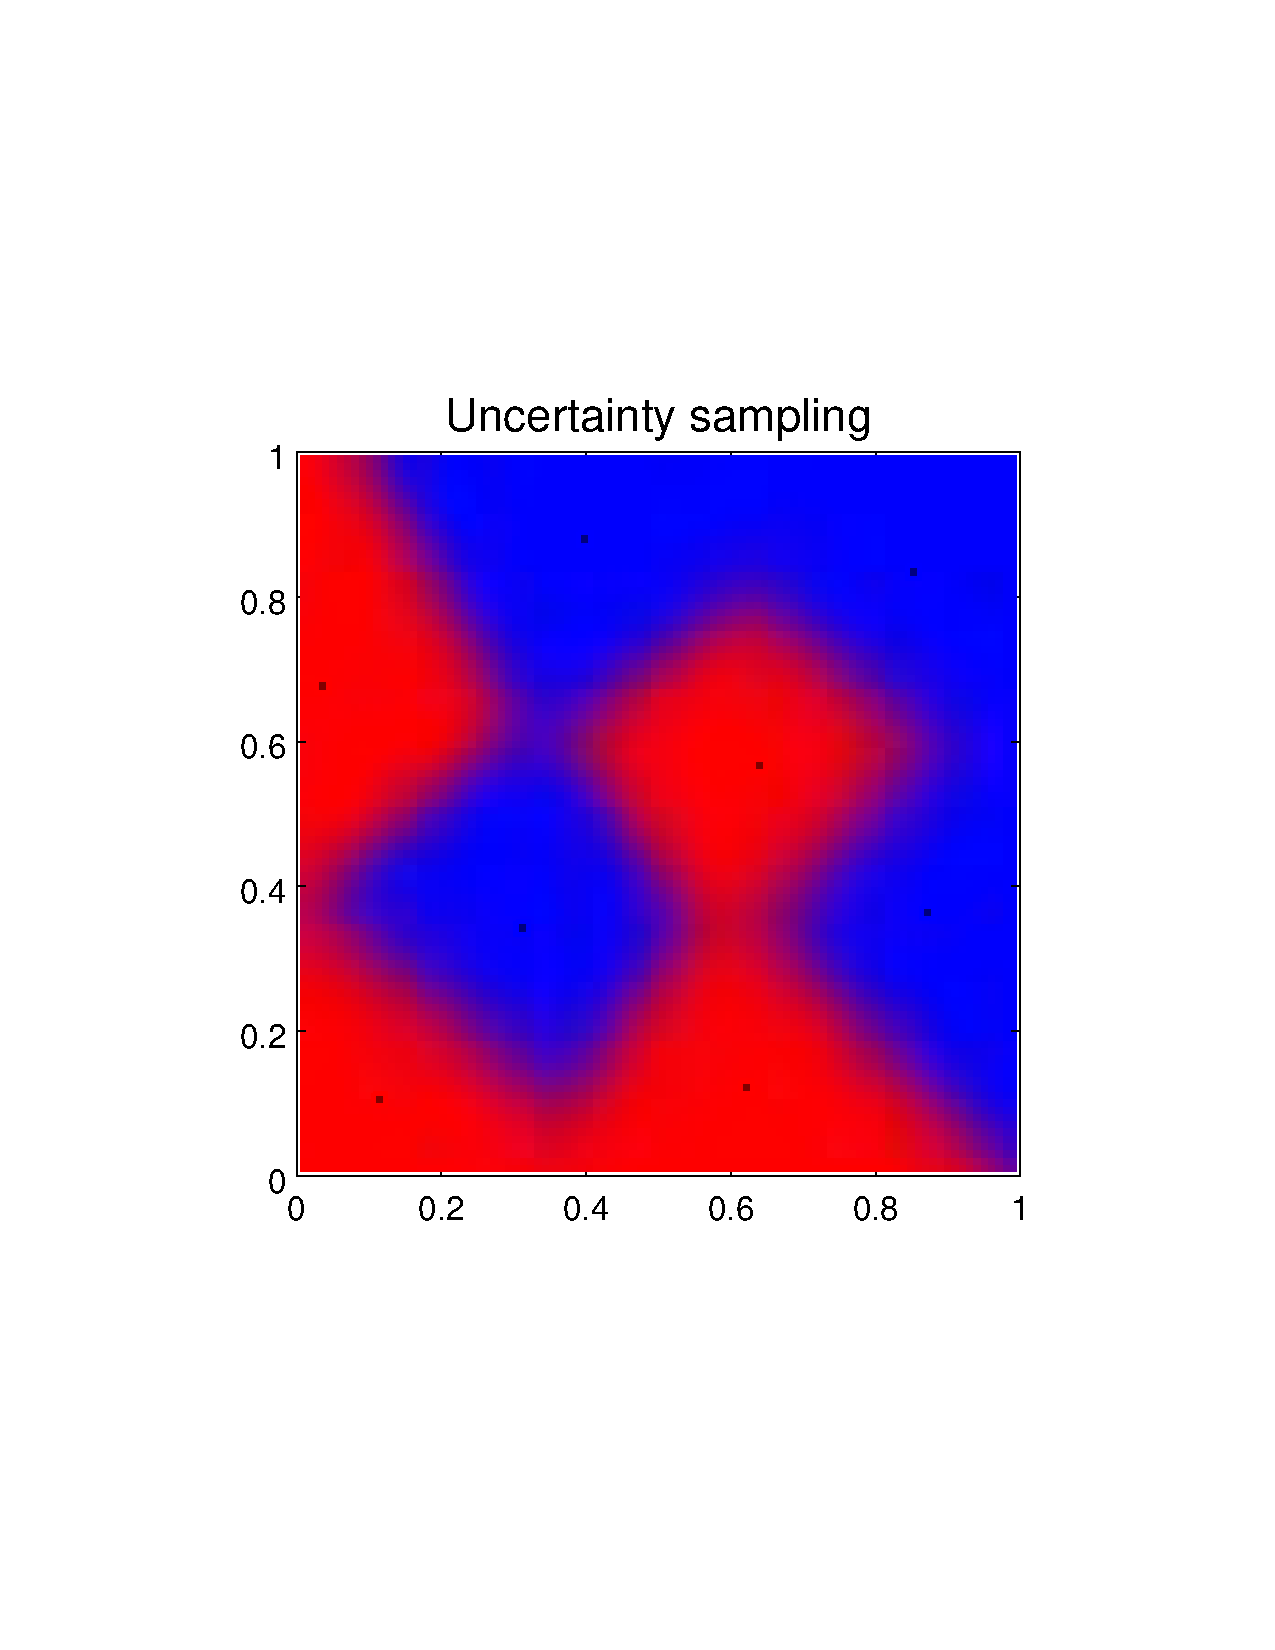
\includegraphics[trim = 4cm 6cm 4cm 4cm, clip = true, width = 0.253\textwidth]{UC16inst}
	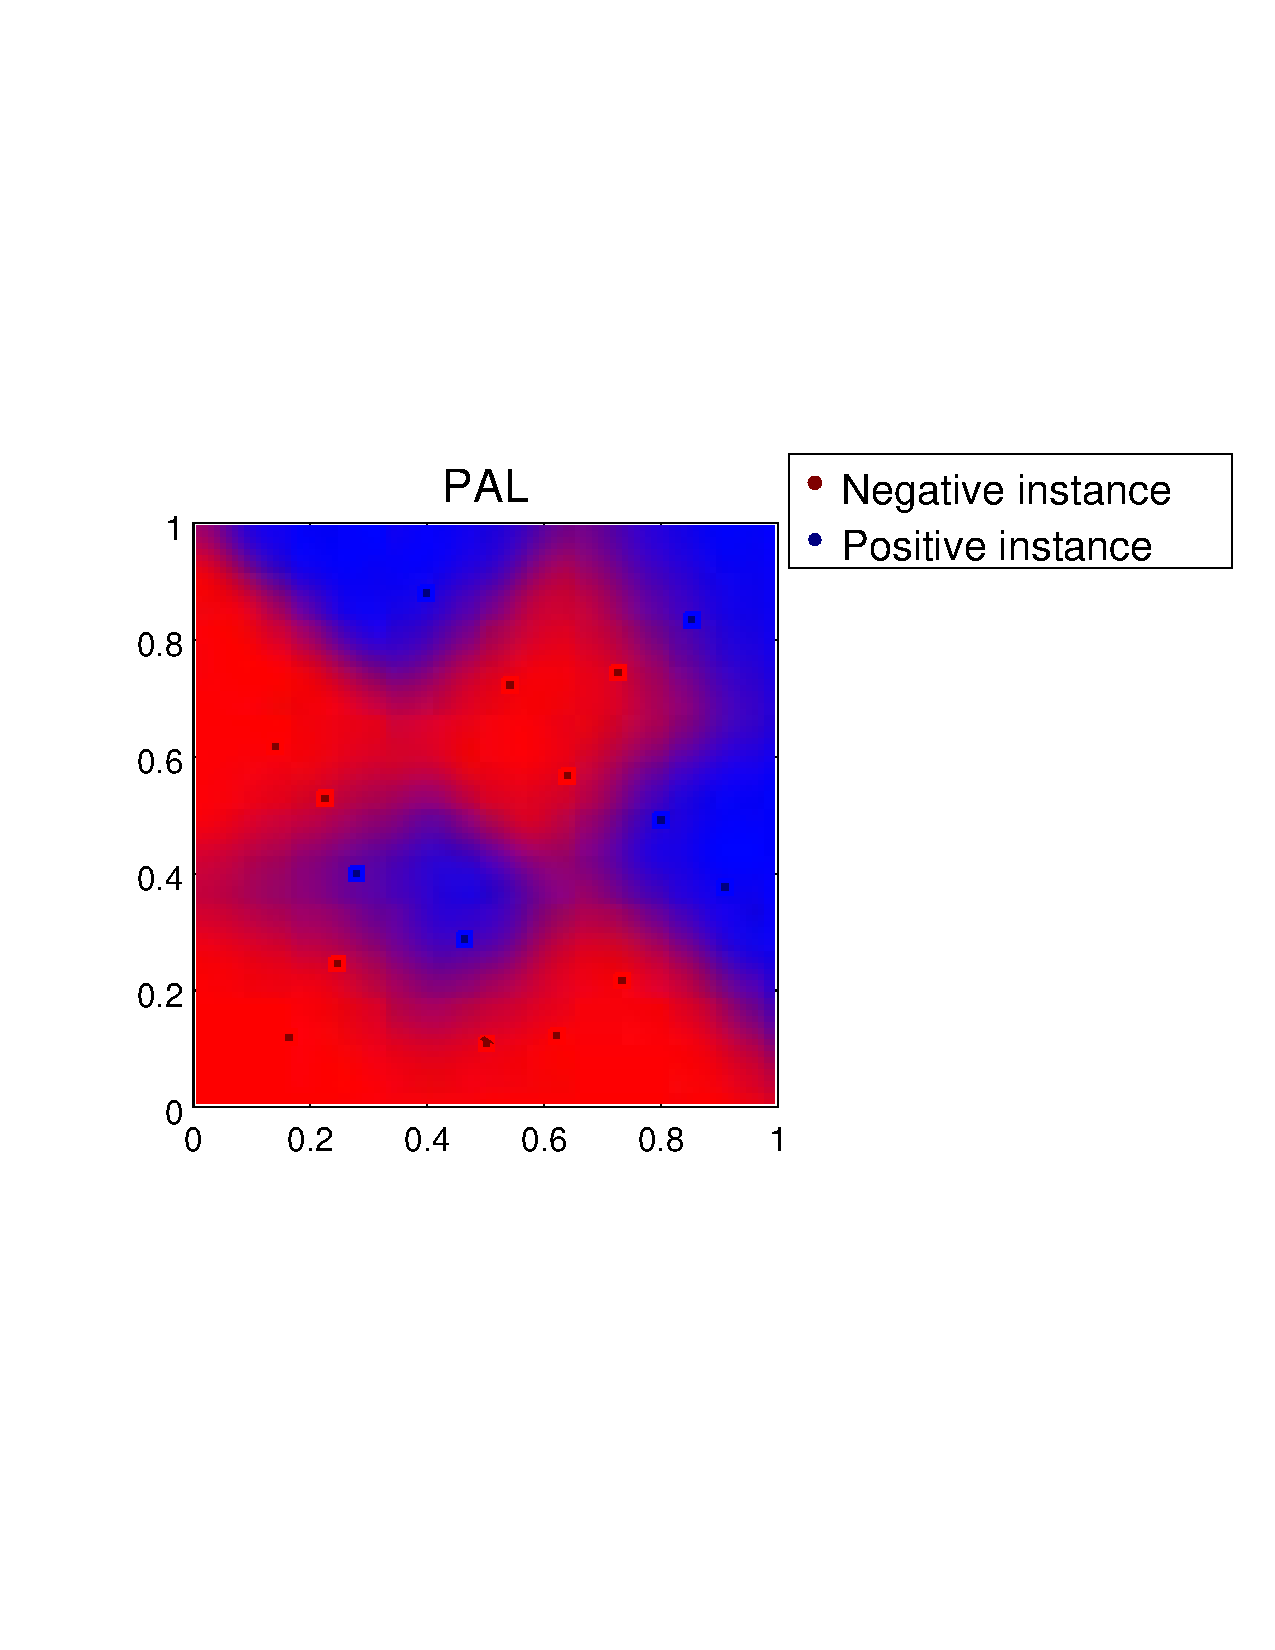
\includegraphics[trim = 2.4cm 6.25cm 0cm 5cm, clip = true, width = 0.37\textwidth]{PAL16inst}
	\caption{Classifier state for random and uncertainty sampling as well as PAL for 16 purchased labels on checke1}
	\label{fig:ALillustration}
\end{figure}

\ref{fig:ALillustration} shows the state of a Parzen-Window classifier (see \ref{evaluation:classifier}) with 16 purchased labels for random sampling, uncertainty sampling and PAL on a 4x4 checkerboard-like dataset with every second field without instances. This structure can be seen fairly well with PAL, which correctly spreads out its purchases over the entire board, while the classifications for random sampling at least resemble its true structure. Uncertainty sampling, however, only purchased labels at the first decision boundary it found and did not bother to look beyond that, resulting in a model that looks nothing like a checkerboard.

\subsection{Model Retraining Improvement and Monte-Carlo-Sampling}
Introduced in \cite{EvansEtAl2015}, \textbf{Model Retraining Improvement (MRI)} is originally intended as a statistically optimal criteria for instance selection in active learning. It does so by selecting the instance which reduces the future loss the most. However, for this it needs an (ideally unbiased) estimate of the future and the initial loss, which the algorithm itself does not provide. Instead, the paper provides a theoretical background for potential future estimators.

Ray and McCallum \cite{RoyEtAl2001} also presents a method to estimate current and future loss of a classifier in an active learning setting, similarly to MRI. They, however, use \textit{Monte-Carlo-Sampling}, resulting in a process comparable to the techniques explained in the next section.

\section{Generalization Performance}
When a learning algorithm is used to induce a classifier, an obvious question is how well said classifier performs or how well it approximates the true target function $f(\vec{x})$. This can be used to select an algorithm when multiple are available or to simply get an estimate on how often the classifier will misclassify data.

To facilitate the calculations further down a closer look at the training set $X_T$ is helpful. As earlier stated, the individual instances are supposed to be independently and identically distributed, which means the set can be seen as a random variable. Now the probability of a specific set depends on the probabilities to draw each of the instances and, in case of supervised and semi-supervised learning, their associated labels. Due to their independence, we can write it as 
\begin{equation}
\label{eq:trainingSet}
p(X_T) = p(\vec{x}_1, y_1) \cdot ... \cdot p(\vec{x}_n, y_n) = \prod_{i=1}^{n} p(\vec{x}_i, y_i)
\end{equation}
A similar formula applies for unsupervised learning. \cite{RodriguezEtAl2013}

\subsection{(Expected) prediction error, training error and loss}
To effectively evaluate the performance of a classifier it is important to quantify when it is mistaken. The \textit{loss function} $L(f(\vec{x}), \hat{f}(\vec{x}))$ describes the error a classifier makes for a specific feature vector. A popular loss function, especially for two-class problems, is \textit{0-1-loss}:
\begin{equation}
L(f(\vec{x}), \hat{f}(\vec{x})) =
\begin{cases}
	0, & \text{if }f(\vec{x}) = \hat{f}(\vec{x}) \\
	1, & \text{else}
\end{cases}
\end{equation}
For regression problems squared or absolute error loss are more effective, since equal function values are improbable in a continuous output space. It seems intuitive to use the feature vectors already used for training again for the performance evaluation, especially since they are already labeled and with that $f(\vec{x})$ for them known. Utilizing the loss function from above, the in-sample error or \textit{training error} \cite{HastieEtAl2009} on the training set $X_T = \{(\vec{x}_1, y_1), ..., (\vec{x}_n, y_n)\}$ is
\begin{equation}
Err_{T} = \frac{1}{N}\sum_{i=1}^{n} L(y_i, \hat{f}(\vec{x}_i))
\end{equation}
If used with the 0-1-loss function, $1 - Err$ is also known as \textit{accuracy}:
\begin{equation}
acc = 1 - err = \frac{|Correct Classifications|}{|Total Classifications|}
\end{equation}

Unfortunately, using the measure to judge a classifier produces a side effect. A learning algorithm which creates a complex classifier that perfectly classifies all training instances will yield a training error of zero. If used on different data points from the same data set, however, an increase in misclassifications will be noted, likely more than for a less complex classifier with a few misclassifications on training data. This phenomenon is known as \textit{overfitting}, resulting from the memorization of $X_T$ by the classifier while a generalization onto the whole data set was wanted \cite{Dietterich1995}.

A more general error measure is the \textit{prediction error}. It draws independent samples from the data distribution $(\mathbf{X}, \mathbf{Y})$ and uses these to examine the loss of a classifier by calculating the expected value over all possible realizations:
\begin{equation}
Err_{S} = E_{(\mathbf{X}, \mathbf{Y})}[L(\mathbf{Y}, \hat{f}(\mathbf{X})) | X_T]
\end{equation}
\cite{RodriguezEtAl2013}. This approach bears a problem: the distribution of our data is usually unknown, hence the need for a classifier. In general, the prediction error cannot be computed directly, thus the need for estimators arises.
An important aspect of the prediction error is the dependence from the fixed training set. This allows for the performance estimation of an already trained classifier. A different approach takes away that dependence and instead calculates the expected error for all possible training sets $Err_{E} = E_{X_T}[Err_{S}]$, which equals
\begin{equation}
Err_{E} = E_{(\mathbf{X}, \mathbf{Y})}[L(\mathbf{Y}, \hat{f}(\mathbf{X}))]
\end{equation}
Using the probability of a specific training set from \ref{eq:trainingSet}, it can also be written as $Err_{E} = \sum_{X_T}^{} p(X_T) \cdot Err_S = \sum_{X_T}^{} Err_S \prod_{i=1}^{|X_T|} p(\vec{x}_i, y_i)$. Here the performance of the algorithm that creates the model $\hat{f}(\vec{x})$ is evaluated, which is no longer of use for the analysis of a trained classifier but can guide the selection of a preferable algorithm, accounting for all possible training sets. Note that we still require knowledge of the underlying distributions for a direct evaluation, realistically making an estimator necessary as well \cite{HastieEtAl2009}.

\subsection{Bias and variance}
In the previous sections we portrayed classifier as a mapping $\hat{f}$ of input values $\vec{x}$ to class labels $y$. Their general task is, however, to assign \textit{probabilities} for each of the possible class labels. Given our random variable $\mathbf{Y}$ for the class labels and a fixed value $\vec{x}$ of our input variable $\mathbf{X}$, $P(\mathbf{Y} = \hat{y} | \vec{x})$ represents the probability that $\mathbf{Y}$ realizes as the value $y$ given our input. Some classifiers, like decision trees, assign a non-zero probability only to one class label given an input, leading to the possibility of being written as a function. In fact, since in practice a definite class label is needed, most classifiers will pick the class label which maximizes said probability, resulting in function-like behaviour anyway \cite{KohaviEtAl1996}.

Another assumption that doesn't necessarily hold was that an error-free target function $f(\vec{x})$ exists. It is entirely possible for our target function to be \textit{noisy}, that is to randomly vary from its true value. In turn, this \textit{variance} leads to blurry class assignments. Thus, we only get a probability $P(\mathbf{Y_T} = y | \vec{x})$ instead of a sharp mapping. Note that the class variable here is different from the one in the previous paragraph; they are conditionally independent for our target distribution and a fixed. Now with this probabilistic notation, it is possible to \textit{decompose} the expected prediction error from the previous section into three components:
\begin{equation}
\begin{split}
Err_{E} &= \sum_{\vec{x}}^{}P(\vec{x})\left(\sigma^2(\vec{x}) + bias^2(\vec{x}) + variance(\vec{x})\right) \\
&= \frac{1}{|X|}\sum_{\vec{x}}^{}\left(\sigma^2(\vec{x}) + bias^2(\vec{x}) + variance(\vec{x})\right)
\end{split}
\end{equation}
The bias and variance express by how much our classifier differs systematically and at random for a given data point from the true value. $\sigma^2$ is the variance of the noise distribution that the target may or may not have; it is the irreducible error that any classifier will always make. The need for the probability of $\vec{x}$ is dropped under the assumption of equal likelihood for all data points \cite{KohaviEtAl1996}. Ideally you would want to minimize both the bias and the variance of your classifier to achieve a low prediction error. Unfortunately, as the model complexity increases to accommodate for more subtle structures in the training data its bias will decrease but the variance will increase. This dilemma is known as the \textit{bias-variance-tradeoff} \cite{KroghVedelsby1995}.

\subsection{Classifier-based estimators}
As stated section 2.2.1, the training error of a classifier usually underestimates the true prediction error $Err_S$. To calculate the desired error, two options are available. Either a direct estimate is taken, usually with dedicated test sets, which will be called \textit{out-of-sample error} since it uses different data points than the training error, or the difference between training and true error is estimated and then added to the training error, also called \textit{optimism}. This section briefly introduces three methods to estimate the optimism: \textit{Akaike information criterion} and \textit{Bayes information criterion}.

The \textbf{Akaike information criterion}(AIC) in its original form was introduced by \cite{Akaike1998} in 1973. It is defined as a function of a model's likelihood and complexity $\lambda$: $AIC = -2 \cdot log(likelihood) + 2\lambda$ \cite{Bozdogan1987}. If instead of a 0-1-loss the log-likelihood-loss is used, a quantity that uses the logarithm of the likelihood of a model given the input, and a linear model with $\lambda$ parameters assumed, the AIC can also be written as
\begin{equation}
AIC = Err_T + 2\frac{\lambda}{n}\sigma^2
\end{equation}
with $n$ as the number of training instances and $\sigma^2$ the variance of the target model \cite{HastieEtAl2009}.

A very similar estimate is the \textbf{Bayesian information criterion}(BIC). Presented by \cite{Schwarz1978} as an alternative to AIC, its definition is similar: $BIC = -2 \cdot log(likelihood) + \lambda log(n)$. It is asymptotically equal to AIC for the size of the training set, but with a steeper penalty for complex models due to the exchange of the factor 2 with $log(n)$ \cite{Weakliem1999}. Using the same assumptions as for AIC, it can be calculated as
\begin{equation}
BIC = \frac{n}{\sigma^2}[Err_T + log(n) \cdot \frac{d}{N}\sigma^2]
\end{equation}

While both criteria are theoretically solid, they are impractical for use in this work; both assume fairly simple model families and restrict the use of loss functions \cite{HastieEtAl2009}.

The third estimator for the optimism is based on the \textbf{Vapnik-Chervonenkis(VC) theory}. In their publication \cite{Vapnik1982} they introduce an algorithm-specific quantity called VC-dimension which is defined as the number of data points a classifier can separate, regardless of their position and class label. Based on this, they derived an upper bound for the optimism of the training error:
\begin{equation}
sup|Err_S - Err_T| \leq 2\frac{ln(\frac{2|X_T|}{h})}{l / h}
\end{equation}
with $h$ as the VC-dimension. The derived bound has some restrictions, however; it is only valid for large training sets and requires knowledge of the VC-dimension. Unfortunately, analytical solutions are known only for a few algorithms and it is not given that it is constant with regard to the training set size \cite{BrumenEtal2004}.

\subsection{Cross-Validation}
As the training error overestimates the classifier performance due to the same samples from the data being used for training as well as evaluation, a different approach is to use separate data for testing. Using this data set called \textit{hold-out set} gives a direct estimate of the prediction error. A common split is to use two thirds of the available (labeled) data as training data and the rest for testing. However, since labeling data can be expensive, often only little labeled data is available. In that case, holding out a third of it may significantly reduce the classifier's performance. An alternative approach is known as \textit{cross-validation} in which the classifier is trained with the full training set. For the performance evaluation the classifier is then retrained with a part of the data, the rest is used for testing \cite{Kohavi1995}.

\textbf{K-fold cross-validation} is the most simple form of cross-validation. Given a set of labeled data $X_T$, $k$ new sets $X_k$ are created, each with size $n$. For each of the $k$ sets a classifier is trained with $X_T \setminus X_k$. $X_k$ then serves as the test set on which the classifier is evaluated, resulting in $k$ estimations of the performance to be expected of the classifier trained with the whole set $X_T$:
\begin{equation}
\widehat{Err}_{S,i} = \frac{1}{n} \sum_{j=1}^{n} L(y_{i, j}, \hat{f}(\vec{x}_{i, j}))
\end{equation}
with $i = \{1, ..., k\}$ \cite{Kohavi1995}. These estimations can be seen as samples of a performance distribution; examples can be uniform (simple average) or beta distribution \cite{KremplEtAl2014}. As a special case of k-fold cross-validation, \textbf{leave-one-out} cross-validation works with test sets of size one. To ensure similarity to the true data distribution, the folds are usually \textit{stratified}; this way the ratio of class labels in $X_T$ is kept also in the test sets.

More expensive variants are \textbf{complete} and \textbf{leave-pair-out} cross-validation. The former uses every possible two-set split of $X_T$ as basis of the estimation, while the latter only regards the possible pairs of data points. Complete cross-validation is rarely used due to its computational complexity \cite{Kohavi1995}, while leave-pair-out seems to strike an acceptable mix of effort and accuracy \cite{PahikkalaEtAl2008}.

\textbf{Leave-p-out} cross-validation generalizes the other variants. Here, every subset of size $p \in \{1, ..., |X_T|-1\}$ is used as a test set, resulting in $|X_T| \choose p$ estimates which are then averaged \cite{ArlotEtAl2010}. Leave-one-out and leave-pair-out are equivalent to leave-p-out with $p = 1$ and $2$, respectively.0

An algorithm specifically designed to work with iterative labeling was introduced by \cite{BrumenEtal2004} under the name of \textit{adaptive incremental k-fold cross validation}. It performs k-fold cross-validation after each increase of the training set size and stops when a certain performance threshold is reached. \cite{AirolaEtAl2001} perform an empirical study of the behaviour for different cross-validation techniques as well as \textit{bootstrapping}, which will be described in the next section. Their findings indicate leave-pair-out and k-fold with $k = 5$ or $10$ with averaged results as the most robust approaches. They also find them to be unbiased performance estimators, which is also stated in \cite{Kohavi1995}. \cite{RodriguezEtAl2013} clarifies that this only holds true for the performance estimation of classifier trained with $n - \frac{n}{k}$ instances. The estimation of classifier performance trained with $n$ samples is afflicted with a \textit{positive error bias}, i.e. the value of the estimated error rate is higher than the true error rate. \cite{EfronEtAl1997}  reinforce this argument with experiments and provide assessment of the variance as well.

\subsection{Bootstrapping}
While closely related to cross-validation, \textbf{bootstrap} takes a slightly different approach. Instead of splitting $X_T$ into mutually exclusive sets, $b$ sets of equal size $n$ are created and filled by random sampling of elements from $X_T$. These are sampled with replacement, meaning can be drawn multiple times into the same set. The classifier is then trained on every bootstrap set $X^b_i$ and tested against the original set $X_T$ \cite{Kohavi1995}:
\begin{equation}
\widehat{Err}^{boot}_i = \frac{1}{|X_T|} \sum_{j=1}^{|X_T|} L(y_j, \hat{f}^b_i(\vec{x}_j))
\end{equation}

Using the whole set $X_T$ as a test set, however, has some unwanted side effects. Because the bootstrap set used to train the classifier and $X_T$ overlap, the classifier's performance is estimated with samples it has already seen in training, leading to a \textit{negative error bias} for the estimated error rate. To avoid this, the bootstrap trained classifiers are only tested on samples which are not part of their training set, known as \textbf{leave-one-out bootstrapping (LOO)} \cite{BorraEtAl2010}:
\begin{equation}
\widehat{Err}^{LOO}_i = \frac{1}{|X_T \setminus X^b_i|} \sum_{(\vec{x}, y) \in X_T \setminus X^b_i}^{} L(y, \hat{f}^b_i(\vec{x}))
\end{equation}

A different bootstrap estimator was introduced by \cite{Efron1983}. While vanilla bootstrap is biased downwards with regard to the estimated error rate, its leave-one-out version goes over the top. The reason for this is similar to the problems of cross-validation: Since the classifier is trained with less instances than available for the estimation, it lacks knowledge that a classifier learned on the full training set has, leading to a worse prediction performance and thus underestimating the performance. As proven by Efron in the same publication, the fraction of unique instances from $X_T$ in a bootstrap set is expected to be $1 - e^{-1} \approx 0.632$. By seeing bootstrapping actually as an estimator for the optimism, similar to AIC and BIC, he derives the so called \textbf{.632 bootstrap}:
\begin{equation}
\widehat{Err}^{.632} = 0.368 \cdot Err_T + 0.632 \cdot \frac{1}{b} \sum_{i=1}^{b} \widehat{Err}^{LOO}_i
\end{equation}
It factors in the training error to lift up the otherwise too conservative estimate of the performance \cite{Efron1983}.

Building on that, \cite{EfronEtAl1997} developed a modified .632 bootstrap under the name of \textbf{.632+ bootstrap}. As their experiments showed, the .632 method has problems estimating the performance of an extremely overfit classifier. To account for this, they use two the two quantities \textit{no-information error rate} and \textit{relative overfitting}. The no-information error rate $\hat{\gamma}$ is defined as as the error rate of a classifier when no dependence exists between input and output data, i.e. $\mathbf{X}$ and $\mathbf{Y}$ are independent. Relative overfitting $\hat{R}$ then expresses how close the classifier is overfit to the no-information error rate:
\begin{equation}
\label{eq:niRate}
\hat{R} =
\begin{cases}
	\frac{\widehat{Err}^{LOO} - Err_T}{\hat{\gamma} - Err_T}, & \text{if } \widehat{Err}^{LOO}, \hat{\gamma} > Err_T \\
	0, & \text{else}
\end{cases}
\end{equation}
The .632+ error rate is then defined as
\begin{equation}
\widehat{Err}^{.632+} = \widehat{Err}^{.632} + \left(min(\widehat{Err}, \hat{\gamma}) - Err_T\right) \cdot \frac{0.368 \cdot 0.632 \cdot \hat{R}}{1 - 0.368 \cdot \hat{R}}
\end{equation}
Part of the assumptions behind this estimator is that leave-one-out bootstrapping has the correct expected error rate value in the case of independence of $\mathbf{X}$ and $\mathbf{Y}$ and a class probability of 0.5 in a 2-class problem, whereas the .632 does not \cite{EfronEtAl1997}. However, \cite{WoodEtAl2007} show in their paper about different error rate estimators that leave-one-out slightly underestimates the error. This stems from the likely inequality of class labels amongst the drawn instances. They show that in such a case, on average, one class is 22\% larger given a random sample. The nearest-neighbour classifier, as assumed by Efron and Tibshirani, assigns an instance the same class label as the closest instance. Since the assumption for the data was that no correlation between feature vector and class label exists, this assignment is random. However, due to the imbalance of class labels, the assignment probabilities are unequal, leading to more classifications for the larger class. In turn, leave-one-out cross-validation will place its error estimate slightly below 0.5. For larger sample sizes this effect is more pronounced; the average class size difference scales with the square root of the sample size. Unfortunately, no experiments with .632+ were performed to evaluate the influence on its estimation performance.

\section{Learning Curves and Regression Models}
The error measures described in section 2.2.1 give an (theoretically) accurate idea about a classifier's performance for either a specific or all possible training sets. In the case of, for instance, active learning, the learning algorithm isn't just fed a single training set. Instead, instances are added iteratively and a new classifier gets trained each round. For this, a representation of the algorithms progress in terms of the resulting classifiers' error rates seems desirable. Originating in the field of psychology, it describes a collection of models to assess the level of comprehension in an individual over the time of exposure or number of examples \cite{Yelle1979}. Similarly, in the context of machine learning it describes a function mapping the size of the training set to a measure of performance; a commonly used measure is accuracy \cite{PerlichEtAl2003}.

As a known functional dependency between accuracy and training set size would enable an easy lookup of the to-be-expected error rate for a certain amount of labeled data, attempts have been made to find a fitting function model.

\subsection{Function families}
The typical form of a learning curve is a steep increase in accuracy when few examples have been presented, leveling more and more for an increased training set, converging towards a maximal accuracy \cite{FigueroaEtal2012}. An example of such a curve can be seen in figure \ref{fig:curve_general}.
\begin{figure}[h]
	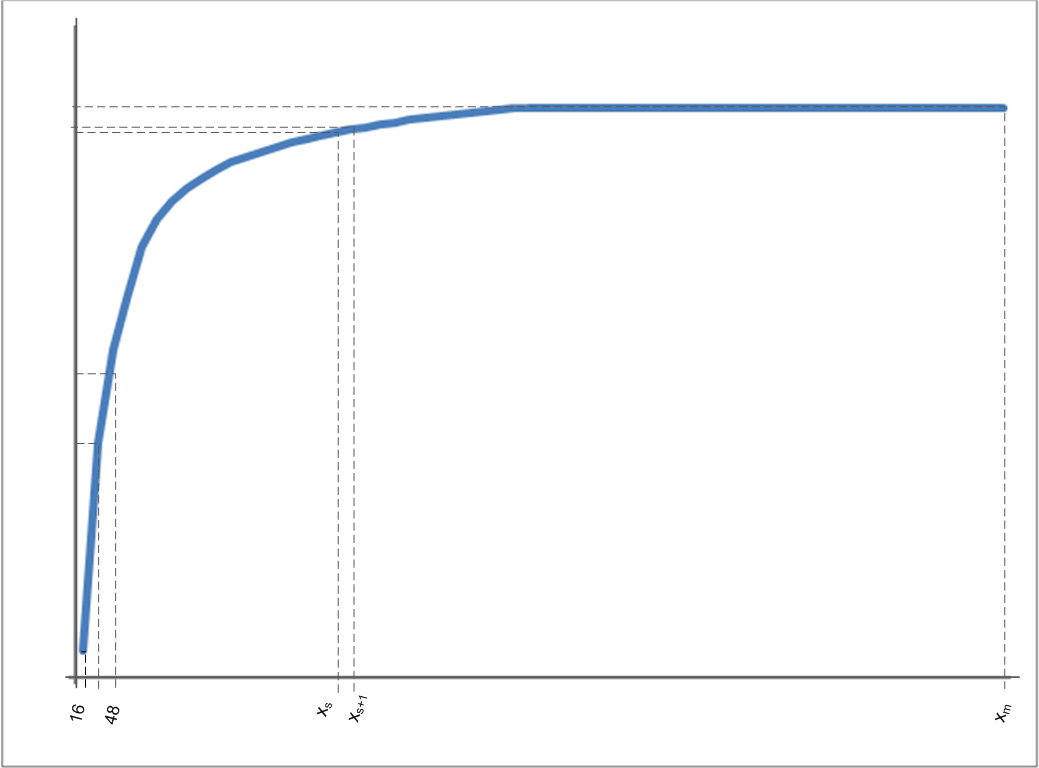
\includegraphics[width = .8\textwidth]{learning_curve_general.png}
	\caption{General appearance of a learning curve. Training set size as x-axis, accuracy as y-axis \cite{FigueroaEtal2012}}
	\label{fig:curve_general}
\end{figure}
Functions families fitting this description are \textbf{power} \cite{FigueroaEtal2012,Singh2005}, \textbf{logarithmic} and \textbf{exponential} \cite{Singh2005}. These papers provide an overview for the fitting of the function types. \cite{Singh2005} uses linear fitting with least squared error as the target and the resulting correlation coefficient as a measure of fitting for four different function models and four classifiers. The power law $f(x) = a + b \cdot x^c$, with $a, b, c$ being regression parameters, performed best on most data sets tested and is also the basis for a proposed method of performance prediction in \cite{FigueroaEtal2012}. It has to be noted, though, that in a fourth of all cases outperforms a linear model the more complex models, mostly on the same data set. This may hint at a data set dependency for the correct curve model.

A related approach is described in \cite{CortesEtal1993}. Here, instead of modeling the prediction error directly, an exponential model is assumed for the optimism of the training error: $Err_S - Err_T = \frac{2b}{|X_T|^\alpha}$ and $Err_S + Err_T = 2a$. Using already acquired (true) error rates, the parameters are estimated from the gradient and amplitude of the data after being transformed into a logarithmic scale and fitted linearly. Extrapolating the function then gives an estimate of the expected error rate for a given $|X_T|$.

\subsection{Maximum-likelihood regression}
Similar to the extrapolation of fitted learning curves, the \textit{maximum-likelihood-regression} presented in \cite{KadieEtal1995}, aims to find the most likely model to explain the given data. Based on this, the model is then extrapolated to obtain an estimate.